\documentclass{beamer}
\mode<presentation>
{
  \usetheme[secheader]{Madrid}
  \setbeamercovered{transparent}
}
\usepackage[utf8]{inputenc}
\usepackage[spanish]{babel}
\usepackage{graphicx}
\usepackage{url}
\usepackage{times}
\usepackage[T1]{fontenc}

\title[Taller Open Source Hardware]{Diseño de Open Source Hardware con ayuda de Software Libre}
%\subtitle{Open Source Hardware}

\author[]{Jorge~Ernesto~Guevara~Cuenca \and Fredy~J.~Pulido~López}

\institute[\url{http://www.altaimpedancia.org}]
{ \inst{1}
  Colibri - Comunidad de Usuarios de Software Libre en Colombia\\
  \url{http://www.slcolombia.org}
  \and
  \inst{2}
  AltaImpedancia\\
  \url{http://www.altaimpedancia.org}
}

\date[Campus Party 2009]
{Campus Party 2009\\Innovación  -  Software Libre}

\subject{Open Source Hardware y Sofware Libre}

\pgfdeclareimage[height=1cm]{logo}{img/altaimpedancia}
\logo{\pgfuseimage{logo}}

\AtBeginSubsection[]
{ \begin{frame}<beamer>{Agenda}
    \tableofcontents[currentsection,currentsubsection]
  \end{frame}}

\beamerdefaultoverlayspecification{<+->}

\begin{document}

\begin{frame}
  \titlepage
\end{frame}

\begin{frame}
  \frametitle{Agenda}%mirar se se puede ir mostrando el diagrama de la metodologia de diseño
  \tableofcontents
  % You might wish to add the option [pausesections]
\end{frame}

\section<presentation>*{Diseño de Open Source Hardware con ayuda de Software Libre}

\begin{frame}
  \frametitle{Objetivo}
  \begin{block}{}
    Desarrollar un ejemplo que permitia a los asistentes entender lo fundamental sobre descripción de hardware mediante lenguajes (HDL) usando Software Libre.
  \end{block}
\end{frame}

\begin{frame}
  \frametitle{Público objetivo y prerequisitos}
  \begin{block}{}
    \begin{itemize}
    \item Personas interesadas en dispositivos lógicos programables desde Linux con Software Libre
    \item Es recomendable tener conocimientos básicos de programación y manejo bsico de consola (DOS).
    \item Llevar el computador con el software previamente instalado. Mirar el manual.
    \end{itemize}
  \end{block}
\end{frame}
 
\begin{frame}
  \frametitle{Introducción}
  \begin{itemize}
  \item Electrónica estática y reconfigurable
    \begin{itemize}
    \item Reconfigurable más adecuada para Open Source Hardware
    \end{itemize}
  \item Que es un PLD - FPGA
  \item Que es un HDL - Verilog HDL
    \begin{itemize}
    \item Se puede hacer descripción estructural y comportamental
    \item Paralelismo
    \end{itemize}
  \item Alcances (FPGA\&HDL) -> Procesadores 
  \end{itemize}
\end{frame}
 
\section{Ejemplo de diseño e implementación}

\subsection{Especificación y revisión de la especificación}

\begin{frame}
  \frametitle{Especificación y revisión de la especificación}
  Campuseros, ustedes son parte de un selecto equipo de personas que tienen como misión implementar un procesador didáctico de 8 bits usando el sistema operativo GNU/Linux y herramientas de Software Libre; para facilitar el desarrollo el proyecto se ha dividido en bloques, y a ustedes les ha sido encargado el diseño e implementación de la Unidad Aritmético Lógica (ALU).
\end{frame}

\begin{frame}
  \frametitle{Especificación y revisión de la especificación}
  \begin{figure}
    \includegraphics[scale=0.3]{img/alu}
  \end{figure}
\end{frame}

\subsection{Selección de Tecnologías y herramientas}

\begin{frame}
  \frametitle{Selección de Tecnologías y herramientas}
  \begin{itemize}
  \item Sistema Operativo Linux
  \item Dispositivo lógico programable fpga de Xilinx (Mejor soportada en linux).
  \item Lenguaje de descripción de hardware Verlog HDL (Mejor soportado por software libre).
  \item Herramienta de desarrollo, editor, cualquiera, el que escoja el diseñador. Nosotros sugerimos
  \end{itemize}
\end{frame}

\subsection{Diseño}

\begin{frame}
  \frametitle{Arquitectura}
  \begin{figure}
    \includegraphics[scale=0.35]{img/alu4}
  \end{figure}
\end{frame}

\begin{frame}
  \frametitle{Arquitectura}
  \begin{table}
    \begin{tabular}{|c c c|l c c c c|}
      \hline
      M&S1&S0&Función&F&X&Y&C0\\
      \hline
       0&0&0&\small{Compl.}&A'&A'&0&0\\
       0&0&1&AND&A AND B&A AND B&0&0\\
       0&1&0&Ident.&A&A&0&0\\
       0&1&1&OR&A OR B&A OR B&0&0\\
       1&0&0&Dec.&A-1&A&Todo unos(1)&0\\
       1&0&1&Suma&A+B&A&B&0\\
       1&1&0&Resta&A+B'+1&A&B'&1\\
       1&1&1&Inc.&A+1&A&Todo ceros(0)&1\\
      \hline
    \end{tabular}
  \end{table}
\end{frame}

\begin{frame}
  \frametitle{Metodología}
  \begin{itemize}
  \item El desarrollo del procesador se dividirá en cuatro partes, el FA, el LE, el AE y la integración de estos.
  \item El FA se desarrollara como ejemplo.
  \item Luego se formarán 2 grupos, uno desarrolla el LE y otro el AE.
  \item Al final se une todo el trabajo para terminar la ALU.
  \end{itemize}
\end{frame}

\begin{frame}
  \frametitle{Ejemplo Sumador (Full Adder - FA)}
  \framesubtitle{Compuertas lógicas}
  \begin{figure}
    \includegraphics[scale=0.25]{img/not}
    \caption{NOT}
  \end{figure}
\end{frame}


\begin{frame}
  \frametitle{Ejemplo Sumador (Full Adder - FA)}
  \framesubtitle{Compuertas lógicas}
  \begin{figure}
    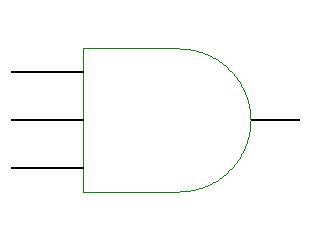
\includegraphics[scale=0.28]{img/and}
    \caption{AND}
  \end{figure}
\end{frame}

\begin{frame}
  \frametitle{Ejemplo Sumador (Full Adder - FA)}
  \framesubtitle{Compuertas lógicas}
  \begin{figure}
    \includegraphics[scale=0.28]{img/or}
    \caption{OR}
  \end{figure}
\end{frame}

\begin{frame}
  \frametitle{Ejemplo Sumador (Full Adder - FA)}
  \framesubtitle{Compuertas lógicas}
  \begin{figure}
    \includegraphics[scale=0.28]{img/xor}
    \caption{XOR}
  \end{figure}
\end{frame}

\begin{frame}
  \frametitle{Ejemplo Sumador (Full Adder - FA)}
  \framesubtitle{Teoría del FA}
  \begin{figure}
    \includegraphics[scale=0.36]{img/sumador}
    \caption{Sumador}
  \end{figure}
\end{frame}

\begin{frame}
  \frametitle{Ejemplo Sumador (Full Adder - FA)}
  \framesubtitle{Implementación del FA en Verilog HDL}
\end{frame}

\subsection{Simulación}

\begin{frame}
  \frametitle{Simulación}
  Simulación del FA con icarus verilog
\end{frame}

\subsection{Revisión del diseño}

\begin{frame}
  \frametitle{Revisión del diseño}
  Comparar salida simulación con tabla de verdad.
\end{frame}

\subsection{Implementación física}

\begin{frame}
  \frametitle{Implementación física}
  Implementar en la fpga el FA. 
\end{frame}

\subsection{Verificación formal}

\begin{frame}
  \frametitle{Verificación formal}
\end{frame}
 
\subsection{Revisión Final}

\begin{frame}
  \frametitle{Revisión Final}
\end{frame}

 \begin{frame}
   \frametitle{Conclusiones}
 \end{frame}

\appendix

\section<presentation>*{Referencias}

\begin{frame}
  \frametitle<presentation>{Bibliografía}
  \begin{thebibliography}{99}
    \beamertemplatebookbibitems
  \bibitem[1]{Gajski}Daniel D. Gajski
    \newblock \emph{Principios de Diseño Digital}
    \newblock Prentice Hall, 1997
  \end{thebibliography}
\end{frame}

%Referencias

\section<presentation>*{Sobre este documento}

\begin{frame}
  \begin{block}{Licencia}
    \begin{figure}
      
\includegraphics[scale=0.9]{img/by-sa}
    \end{figure}
    \centering
    \small Creative Commons Atribución-Compartir Obras Derivadas Igual 2.5 Colombia
    \small \url{http://creativecommons.org/licenses/by-sa/2.5/co}
\end{block}
\begin{block}{}
  Creado con \LaTeX/Beamer
\end{block}
\end{frame}

\end{document}
